\documentclass[12pt]{article}
\usepackage[utf8]{inputenc}
\usepackage[spanish, mexico]{babel}
\usepackage[T1]{fontenc}
\usepackage{Alegreya}
\usepackage{euler}
\usepackage{amssymb}
\usepackage{amsmath}
\usepackage{multirow}
\usepackage{blkarray}
\usepackage{booktabs}
\usepackage{graphicx}
\usepackage{caption}
\usepackage{subcaption}
\usepackage[dvipsnames]{xcolor}
\usepackage{colortbl}
\usepackage{tikz}
\usepackage{hyperref}
\usepackage{geometry}

\geometry{
  top=10mm,
  bottom=10mm,
  left=10mm,
  right=10mm
}

\usetikzlibrary{positioning, shapes.geometric}

\graphicspath{{./images/}}

\makeatletter
\def\@maketitle{
  \hbox{
    \noindent
    \begin{minipage}{\textwidth}
      \hbox{\rule{\textwidth}{2pt}}
      \smallskip
      \begin{center}
        {\large\@title}
      \end{center}
      \medskip
      \@author\textsuperscript{1}, \Iauthor\textsuperscript{1}\\
                              {\footnotesize 1. \textit{Facultad de Ciencias, Universidad Nacional Autónoma de México, Ciudad Universitaria, Coyoacán 04510, CDMX, México}}\\
                              \hbox{\rule{\textwidth}{1pt}}
    \end{minipage}
  }\medskip
}
\makeatother

\title{Análisis de un algoritmo más eficiente para determinar la similitud entre genomas con un enfoque en la teoría de gráficas}
\author{José Guadalupe de Jesús Marín Parra}
\newcommand{\Iauthor}{Erik Rangel Limón}

\begin{document}

\pagenumbering{gobble}

\maketitle

\section{Introducción}

\noindent La matriz de distancias de distintos pares de genoma han sido clave para el análisis filogenético de las especies, por lo general la matriz de distancias de $n$ especies es una matriz $n\times n$ tal que toda entrada $a_{ij}$ determina un valor que representa qué tan lejana es la especie $i$ de la especie $j$; una especie muy parecida a otra tendrá un valor menor en su entrada (si son la misma, entonces será 0), y mientras más distintas sean, este valor crecerá.

Hay muchas formas de crear ésta matriz de distancias, una de las más comunes es mediante los algoritmos de alineamiento de secuencias, sin embargo éstos algoritmos tienen una complejidad considerablemente alta, tan sólo la propuesta de \textit{Needleman-Wunsch} toma tiempo $O(nm)$ siendo $n$ y $m$ el tamaño de dos secuencias respectivamente, por lo que si queremos analizar dos secuencias de una misma especie, ésto tomaría tiempo $O(n^2)$, lo cual haría muy ineficiente crear una matriz de distancias que contempla todas las comparaciones posibles entre dos especies.

Es posible crear una matriz de distancias prescindiendo del algoritmo de alineamiento, usando un algoritmo enfocado en la teoría de gráficas propuesto en el artículo \textit{A new graph-theoretic approach to determine the similarity of genome sequences based on nucletide triplets}\textsuperscript{1}, en donde la comparación de dos secuencias toma tiempo $O(n)$ siendo $n$ la mayor de las secuencias según su longitud.

Este método permite que la matriz de distancias pueda ser creada con diversas secuencias en un tiempo considerablemente menor que usando cualquier algoritmo de alineamiento.

La idea de usar gráficas de manera general se utiliza para contar los distintos tripletes de nucleótidos que hay en una secuencia, lo cual puede ser útil para muchos otros usos.

\subsection{Objetivos}

\begin{itemize}
\item Repasaremos algunas definiciones que utilizaremos sobre la teoría de gráficas.
\item Describiremos el funcionamiento del algoritmo.
\item Compararemos la complejidad de la creación de la matriz de distancias utilizando el algoritmo de alineamiento con la creación de la misma utilizando el algoritmo enfocado en gráficas.
\item Implementaremos el algoritmo.
\item Probaremos el algoritmo para crear el arbol filogenético de varias especies por medio del algoritmo UPGMA.\@
\end{itemize}

\section{Métodos}

\noindent El algoritmo enfocado a la teoría de gráficas es un método muy conveniente para analizar secuencias, en éste usamos lo que se llama una gráfica bipartita completa $K_{16,4}$ para modelar todos los posibles tripletes de nucléotidos.

La base de éste algoritmo es crear una gráfica bipartita para cada secuencia que queramos analizar, y a cada una de las aristas les asignaremos un peso según el número de veces que aparezca el tri-nucleótido modelado por la arista.

\newpage

\subsection{Sobre teoría de gráficas}

\noindent Una gráfica es un par ordenado $(V,A)$ donde $V$ es el conjunto de vértices y $A$ es un conjunto de aristas. El conjunto de aristas puede modelar una relación arbitraria simétrica y no reflexiva entre dos vértices de $V$ (recordemos que la simetría en una relación $\mathcal{R}$ quiere decir que $\forall_{a,b}a\mathcal{R}b\Rightarrow b\mathcal{R}a$, y reflexividad es que $\forall_a a\mathcal{R}a$); por lo tanto para una relación arbitrariaria $\mathcal{R}$ entre los vértices de $V$, podemos definir al conjunto de aristas como sigue:

\[A=\{uv\ |\ u,v\in V, u\mathcal{R}v\}\]

\begin{figure}[h!]
  \centering
  \begin{subfigure}[b]{0.3\textwidth}
    \centering
    \begin{tikzpicture}[
        vx/.style={circle,draw},
        node distance=2cm
      ]
      \def\ngon{3}
      \node[regular polygon,regular polygon sides=\ngon,minimum size=4cm] (v) {};
      \foreach\x in {1,...,\ngon}{\node[vx] (v\x) at (v.corner \x) {$v_{\x}$};}
      \foreach\i in {1,...,\ngon}{
        \foreach\j in {\i,...,\ngon}{\draw (v\i) -- (v\j);}
      }
    \end{tikzpicture}
    \caption{Gráfica $G$}
  \end{subfigure}
  \hfil
  \begin{subfigure}[b]{0.3\textwidth}
    \centering
    \begin{tikzpicture}[
        vx/.style={circle,draw},
        node distance=2cm,
      ]
      \def\ngon{4}
      \node[regular polygon,regular polygon sides=\ngon,minimum size=4cm] (v) {};
      \foreach\x in {1,...,\ngon}{\node[vx] (v\x) at (v.corner \x) {$v_{\x}$};}
      \node[vx] (v0) at (v.center) {$v_0$};
      \draw (v0) -- (v3);
      \draw (v0) -- (v4);
      \draw (v3) -- (v4);
      \draw (v3) -- (v2);
      \draw (v4) -- (v1);
    \end{tikzpicture}
    \caption{Gráfica $H$}
  \end{subfigure}
  \caption{Ejemplos de gráficas cualesquiera}
\end{figure}

Sabiendo ésto, recordaremos algunas definiciones sobre teoría de gráficas que utilizaremos en el algoritmo:

\begin{itemize}
\item Dada una gráfica $G$, denotaremos como $V(G)$ a su conjunto de vértices, y denotaremos como $A(G)$ a su conjunto de aristas.
\item Sean $u,v\in V(G)$ diremos que $u$ y $v$ son \textit{adyacentes} si y sólo si existe la arista $uv\in A(G)$.

  \begin{figure}[h!]
    \centering
    \begin{subfigure}[b]{0.3\textwidth}
      \centering
      \begin{tikzpicture}[
          vx/.style={circle,draw},
          node distance=2cm
        ]
        \node[vx] (u) {u};
        \node[vx] (v) [right of=u] {v};
        \draw (u) -- (v);
      \end{tikzpicture}
      \caption{Los vértices $u$ y $v$ son \textit{adyacentes}}
    \end{subfigure}
    \hfil
    \begin{subfigure}[b]{0.3\textwidth}
      \centering
      \begin{tikzpicture}[
          vx/.style={circle,draw},
          node distance=2cm
        ]
        \node[vx] (w) {w};
        \node[vx] (y) [right of=w] {y};
      \end{tikzpicture}
      \caption{Los vértices $w$ y $y$ \textbf{no} son \textit{adyacentes}}
    \end{subfigure}
    \caption{Ejemplos de adyacencias}
  \end{figure}
  
\item Sea $A$ un subconjunto de $V(G)$, diremos que $A$ es un \textit{conjunto independiente de vértices} si y sólo si para todo par de vértices $u,v\in A$, $u$ y $v$ \textbf{no} son adyacentes.

  \begin{figure}[h!]
    \centering
    \begin{tikzpicture}[
        vx/.style={circle,draw},
        node distance=2cm,
      ]
      \def\ngon{4}
      \node[regular polygon,regular polygon sides=\ngon,minimum size=4cm] (v) {};
      \foreach\x in {1,...,\ngon}{\node[vx] (v\x) at (v.corner \x) {$v_{\x}$};}
      \node[vx] (v0) at (v.center) {$v_0$};
      \draw (v0) -- (v3);
      \draw (v0) -- (v4);
      \draw (v3) -- (v4);
      \draw (v3) -- (v2);
      \draw (v4) -- (v1);
    \end{tikzpicture}
    \caption{$\{v_0,v_1,v_2\}$ es un \textit{conjunto independiente}, pues no existen adyacencias entre ellos}
  \end{figure}

  \newpage
  
\item Diremos que una gráfica $G$ es \textit{bipartita} si y sólo si existe una partición de $V(G)$ en dos conjuntos $V_1$, $V_2$ tales que $V_1$ y $V_2$ son \textit{conjuntos independientes de vértices}.

  \begin{figure}[h!]
    \centering
    \begin{tikzpicture}[
        vx/.style={circle,draw},
        node distance=2cm
      ]
      \node[vx] (u) {u};
      \node[vx] (v) [below of=u] {v};
      \node[vx] (w) [below of=v] {w};
      \node[vx] (x) [right=2cm of u] {x};
      \node[vx] (y) [below of=x] {y};
      \node[vx] (z) [below of=y] {z};
      \draw (u) -- (y);
      \draw (u) -- (z);
      \draw (v) -- (x);
      \draw (v) -- (y);
      \draw (w) -- (z);
    \end{tikzpicture}
    \caption{Ejemplo de gráfica \textit{bipartita}. $V_1=\{u,v,w\}$ y $V_2=\{x,y,z\}$}    
  \end{figure}
  
\item Una gráfica es \textit{completa} si y sólo si para todo par de vértices $u,v\in V(G)$, $u$ y $v$ son adyacentes. Éstas serán denotaras por $K_n$, con $n$ el número de vértices.

  \begin{figure}[h!]
    \centering
    \begin{subfigure}[b]{0.3\textwidth}
      \centering
      \begin{tikzpicture}[
          vx/.style={circle,draw}
        ]
        \def\ngon{3}
        \node[regular polygon,regular polygon sides=\ngon,minimum size=3cm] (v) {};
        \foreach\x in {1,...,\ngon}{\node[vx] (v\x) at (v.corner \x) {$v_{\x}$};}
        \foreach\i in {1,...,\ngon}{
          \foreach\j in {\i,...,\ngon}{\draw (v\i) -- (v\j);}
        }
      \end{tikzpicture}
      \caption{Gráfica $K_3$}
    \end{subfigure}
    \hfil
    \begin{subfigure}[b]{0.3\textwidth}
      \centering
      \begin{tikzpicture}[
          vx/.style={circle,draw}
        ]
        \def\ngon{5}
        \node[regular polygon,regular polygon sides=\ngon,minimum size=3cm] (v) {};
        \foreach\x in {1,...,\ngon}{\node[vx] (v\x) at (v.corner \x) {$v_{\x}$};}
        \foreach\i in {1,...,\ngon}{
          \foreach\j in {\i,...,\ngon}{\draw (v\i) -- (v\j);}
        }
      \end{tikzpicture}
      \caption{Gráfica $K_5$}
    \end{subfigure}
    \hfil
    \begin{subfigure}[b]{0.3\textwidth}
      \centering
      \begin{tikzpicture}[
          vx/.style={circle,draw}
        ]
        \def\ngon{7}
        \node[regular polygon,regular polygon sides=\ngon,minimum size=3cm] (v) {};
        \foreach\x in {1,...,\ngon}{\node[vx] (v\x) at (v.corner \x) {$v_{\x}$};}
        \foreach\i in {1,...,\ngon}{
          \foreach\j in {\i,...,\ngon}{\draw (v\i) -- (v\j);}
        }
      \end{tikzpicture}
      \caption{Gráfica $K_7$}
    \end{subfigure}
    \caption{Ejemplos de gráficas $K_n$}
  \end{figure}
  
\item Una gráfica será \textit{bipartita completa} si y sólo si la gráfica es bipartita por dos conjuntos $V_1,V_2$ y además para todo vértice $u\in V_1$, $u$ es adyacente a todo vértice $v\in V_2$. Esta gráfica se denotará como $K_{i,j}$ siendo $i$ la cardinalidad de $V_1$ y $j$ la cardinalidad de $V_2$.

  \begin{figure}[h!]
    \centering
    \begin{tikzpicture}[
        vx/.style={circle,draw},
        node distance=2cm
      ]
      \node[vx] (u) {u};
      \node[vx] (v) [below of=u] {v};
      \node[vx] (w) [below of=v] {w};
      \node[vx] (x) [right=2cm of u] {x};
      \node[vx] (y) [below of=x] {y};
      \node[vx] (z) [below of=y] {z};
      \draw (u) -- (x);
      \draw (u) -- (y);
      \draw (u) -- (z);
      \draw (v) -- (x);
      \draw (v) -- (y);
      \draw (v) -- (z);
      \draw (w) -- (x);
      \draw (w) -- (y);
      \draw (w) -- (z);
    \end{tikzpicture}
    \caption{Ejemplo de gráfica \textit{bipartita completa} $K_{3,3}$}    
  \end{figure}

  \newpage
  
\item Para denotar el peso que va a tener una arista en una gráfica $G$, se tiene que definir una función $w:A(G)\rightarrow\mathbb{R}$.

  \begin{figure}[h!]
    \centering
    \begin{tikzpicture}[
        vx/.style={circle,draw},
        node distance=3cm
      ]
      \node[vx] (u) {u};
      \node[vx] (v) [right of=u] {v};
      \draw (u) to node [anchor=south] {$3$} (v);
    \end{tikzpicture}
    \caption{Ejemplo de peso de una arista $w(uv)=3$}
  \end{figure}
  
\item La matriz de adyacencias de una gráfica $G$, digamos $M$, será una matriz bidimensional $n\times n$ siendo $n$ el número de vértices de $G$, si los vértices son $V(G)=\{v_1,\ldots,v_n\}$, la entrada $M_{ij}$ de la matriz sera $1$ si y sólo si $v_i v_j\in A(G)$, y será $0$ en cualquier otro caso.

  \begin{figure}[h!]
    \centering
    \begin{subfigure}[b]{0.3\textwidth}
      \centering
      \begin{tikzpicture}[
          vx/.style={circle,draw},
          node distance=2cm,
        ]
        \def\ngon{4}
        \node[regular polygon,regular polygon sides=\ngon,minimum size=4cm] (v) {};
        \foreach\x in {1,...,\ngon}{\node[vx] (v\x) at (v.corner \x) {$v_{\x}$};}
        \node[vx] (v0) at (v.center) {$v_0$};
        \draw (v0) -- (v3);
        \draw (v0) -- (v4);
        \draw (v3) -- (v4);
        \draw (v3) -- (v2);
        \draw (v4) -- (v1);
      \end{tikzpicture}
      \caption{Gráfica $G$}
    \end{subfigure}
    \hfil
    \begin{subfigure}[b]{0.3\textwidth}
      \centering
      \begin{blockarray}{cccccc}
        & $v_0$ & $v_1$ & $v_2$ & $v_3$ & $v_4$\\
        \begin{block}{c (ccccc)}
          $v_0$ & $0$ & $0$ & $0$ & $1$ & $1$\\
          $v_1$ & $0$ & $0$ & $0$ & $0$ & $1$\\
          $v_2$ & $0$ & $0$ & $0$ & $1$ & $0$\\
          $v_3$ & $1$ & $0$ & $1$ & $0$ & $1$\\
          $v_4$ & $1$ & $1$ & $0$ & $1$ & $0$\\
        \end{block}
      \end{blockarray}
      \caption{Matriz de adyacencias de $G$}
    \end{subfigure}
    \caption{Ejemplo de matriz de adyacencias}
  \end{figure}
  
\item La matriz de adyacencias de una gráfica bipartita por conjuntos independientes $V_1$ y $V_2$ se puede reducir a una matriz de tamaño $|V_1|\times|V_2|$, dado que sabemos que entre los vértices de $V_1$ nunca habrá una adyacencia, y tampoco entre los vértices de $|V_2|$. De esta manera, la matriz de adyacencia reducida de una gráfica \textit{bipartita completa} será una matriz que tiene $1$ en todas sus entradas.

  \begin{figure}[h!]
    \centering
    \begin{subfigure}[b]{0.3\textwidth}
      \centering
      \begin{tikzpicture}[
          vx/.style={circle,draw},
          node distance=1.5cm
        ]
        \node[vx] (u) {u};
        \node[vx] (v) [below of=u] {v};
        \node[vx] (w) [below of=v] {w};
        \node[vx] (x) [right=1.5cm of u] {x};
        \node[vx] (y) [below of=x] {y};
        \node[vx] (z) [below of=y] {z};
        \draw (u) -- (y);
        \draw (u) -- (z);
        \draw (v) -- (x);
        \draw (v) -- (y);
        \draw (w) -- (z);
      \end{tikzpicture}
      \caption{Gráfica \textit{bipartita}}
    \end{subfigure}
    \hfil
    \begin{subfigure}[b]{0.3\textwidth}
      \centering
      \begin{blockarray}{cccc}
        & x & y & z\\
        \begin{block}{c (ccc)}
          u & $0$ & $1$ & $1$\\
          v & $1$ & $1$ & $0$\\
          w & $0$ & $0$ & $1$\\
        \end{block}
      \end{blockarray}
      \caption{Matriz de adyacencias reducida}
    \end{subfigure}
    \caption{Ejemplo de gráfica \textit{bipartita} y su respectiva matriz de adyacencias reducida.}    
  \end{figure}
  
\end{itemize}

\subsection{Conteo de tri-nucleótidos por medio de gráficas}

Lo que hacemos en éste algoritmo es utilizar una gráfica $K_{16,4}$ que representan a todos los tripletes de nucléotidos, en donde el conjunto independiente de 16 vértices son todas las posibles formas de tener una cadena con dos caracteres de ``A'', ``C'', ``T'' o ``G''; mientras que el conjunto de 4 vértices son cada uno de los caracteres mencionados anteriormente.

De forma visual, podemos ver a la gráfica mencionada como sigue:

\newpage

\begin{figure}[h!]
  \centering
  \begin{tikzpicture}[
      vx/.style={circle,draw}
    ]
    \node[vx] (aa) {AA};
    \node[vx] (ac) [below=2.5mm of aa] {AC};
    \node[vx] (at) [below=2.5mm of ac] {AT};
    \node[vx] (ag) [below=2.5mm of at] {AG};
    \node[vx] (ca) [below=2.5mm of ag] {CA};
    \node[vx] (cc) [below=2.5mm of ca] {CC};
    \node[vx] (ct) [below=2.5mm of cc] {CT};
    \node[vx] (cg) [below=2.5mm of ct] {CG};
    \node[vx] (ta) [below=2.5mm of cg] {TA};
    \node[vx] (tc) [below=2.5mm of ta] {TC};
    \node[vx] (tt) [below=2.5mm of tc] {TT};
    \node[vx] (tg) [below=2.5mm of tt] {TG};
    \node[vx] (ga) [below=2.5mm of tg] {GA};
    \node[vx] (gc) [below=2.5mm of ga] {GC};
    \node[vx] (gt) [below=2.5mm of gc] {GT};
    \node[vx] (gg) [below=2.5mm of gt] {GG};
    \node[vx] (a) [below right=0.7mm and 8cm of ac] {A};
    \node[vx] (c) [below right=0.7mm and 8cm of cc] {C};
    \node[vx] (t) [below right=0.7mm and 8cm of tc] {T};
    \node[vx] (g) [below right=0.7mm and 8cm of gc] {G};
    \draw (a) edge[OrangeRed, thick] (aa);
    \draw (a) edge[OrangeRed, thick] (ac);
    \draw (a) edge[OrangeRed, thick] (at);
    \draw (a) edge[OrangeRed, thick] (ag);
    \draw (a) edge[Blue, thick] (ca);
    \draw (a) edge[Blue, thick] (cc);
    \draw (a) edge[Blue, thick] (ct);
    \draw (a) edge[Blue, thick] (cg);
    \draw (a) edge[Orchid, thick] (ta);
    \draw (a) edge[Orchid, thick] (tc);
    \draw (a) edge[Orchid, thick] (tt);
    \draw (a) edge[Orchid, thick] (tg);
    \draw (a) edge[LimeGreen, thick] (ga);
    \draw (a) edge[LimeGreen, thick] (gc);
    \draw (a) edge[LimeGreen, thick] (gt);
    \draw (a) edge[LimeGreen, thick] (gg);
    \draw (c) edge[RedOrange, thick] (aa);
    \draw (c) edge[RedOrange, thick] (ac);
    \draw (c) edge[RedOrange, thick] (at);
    \draw (c) edge[RedOrange, thick] (ag);
    \draw (c) edge[RoyalPurple, thick] (ca);
    \draw (c) edge[RoyalPurple, thick] (cc);
    \draw (c) edge[RoyalPurple, thick] (ct);
    \draw (c) edge[RoyalPurple, thick] (cg);
    \draw (c) edge[Thistle, thick] (ta);
    \draw (c) edge[Thistle, thick] (tc);
    \draw (c) edge[Thistle, thick] (tt);
    \draw (c) edge[Thistle, thick] (tg);
    \draw (c) edge[Green, thick] (ga);
    \draw (c) edge[Green, thick] (gc);
    \draw (c) edge[Green, thick] (gt);
    \draw (c) edge[Green, thick] (gg);
    \draw (t) edge[BrickRed, thick] (aa);
    \draw (t) edge[BrickRed, thick] (ac);
    \draw (t) edge[BrickRed, thick] (at);
    \draw (t) edge[BrickRed, thick] (ag);
    \draw (t) edge[MidnightBlue, thick] (ca);
    \draw (t) edge[MidnightBlue, thick] (cc);
    \draw (t) edge[MidnightBlue, thick] (ct);
    \draw (t) edge[MidnightBlue, thick] (cg);
    \draw (t) edge[Yellow, thick] (ta);
    \draw (t) edge[Yellow, thick] (tc);
    \draw (t) edge[Yellow, thick] (tt);
    \draw (t) edge[Yellow, thick] (tg);
    \draw (t) edge[SeaGreen, thick] (ga);
    \draw (t) edge[SeaGreen, thick] (gc);
    \draw (t) edge[SeaGreen, thick] (gt);
    \draw (t) edge[SeaGreen, thick] (gg);
    \draw (g) edge[Peach, thick] (aa);
    \draw (g) edge[Peach, thick] (ac);
    \draw (g) edge[Peach, thick] (at);
    \draw (g) edge[Peach, thick] (ag);
    \draw (g) edge[WildStrawberry, thick] (ca);
    \draw (g) edge[WildStrawberry, thick] (cc);
    \draw (g) edge[WildStrawberry, thick] (ct);
    \draw (g) edge[WildStrawberry, thick] (cg);
    \draw (g) edge[Maroon, thick] (ta);
    \draw (g) edge[Maroon, thick] (tc);
    \draw (g) edge[Maroon, thick] (tt);
    \draw (g) edge[Maroon, thick] (tg);
    \draw (g) edge[Plum, thick] (ga);
    \draw (g) edge[Plum, thick] (gc);
    \draw (g) edge[Plum, thick] (gt);
    \draw (g) edge[Plum, thick] (gg);
  \end{tikzpicture}
  \caption{Gráfica bipartita de posibles tripletes de nucleótidos (Los colores sólo son para diferenciar mejor a las aristas)}
\end{figure}

De esta manera, para cada secuencia que queramos analizar, generaremos una matriz de tamaño $16\times 4$, que representaría la matriz de adyacencias reducida de la gráfica bipartita de posibles tripletes de nucleótidos; sin embargo, como todas las entradas serían iguales, llenaremos dicha matriz con el peso de la arista que representa cada entrada.

Como dijimos anteriormente, el peso de la arista representará las veces que aparece dicho tri-nucleótido en la secuencia, y además no consideraremos la posición en la que se encuentra. Por ejemplo, veamos cuál sería el peso de las aristas en la subsecuencia hipotética ``ACCTGATTGGAC''.

\newpage

\begin{table}[h!]
  \centering
  \begin{tabular}{cccccccccccc}
    A & C & C & T & G & A & T & T & G & G & A & C\\
    \midrule
    A & C & C & $\cdot$ & $\cdot$ & $\cdot$ & $\cdot$ & $\cdot$ & $\cdot$ & $\cdot$ & $\cdot$ & $\cdot$\\
    $\cdot$ & C & C & T & $\cdot$ & $\cdot$ & $\cdot$ & $\cdot$ & $\cdot$ & $\cdot$ & $\cdot$ & $\cdot$\\
    $\cdot$ & $\cdot$ & C & T & G & $\cdot$ & $\cdot$ & $\cdot$ & $\cdot$ & $\cdot$ & $\cdot$ & $\cdot$\\
    $\cdot$ & $\cdot$ & $\cdot$ & T & G & A & $\cdot$ & $\cdot$ & $\cdot$ & $\cdot$ & $\cdot$ & $\cdot$\\
    $\cdot$ & $\cdot$ & $\cdot$ & $\cdot$ & G & A & T & $\cdot$ & $\cdot$ & $\cdot$ & $\cdot$ & $\cdot$\\
    $\cdot$ & $\cdot$ & $\cdot$ & $\cdot$ & $\cdot$ & A & T & T & $\cdot$ & $\cdot$ & $\cdot$ & $\cdot$\\
    $\cdot$ & $\cdot$ & $\cdot$ & $\cdot$ & $\cdot$ & $\cdot$ & T & T & G & $\cdot$ & $\cdot$ & $\cdot$\\
    $\cdot$ & $\cdot$ & $\cdot$ & $\cdot$ & $\cdot$ & $\cdot$ & $\cdot$ & T & G & G & $\cdot$ & $\cdot$\\
    $\cdot$ & $\cdot$ & $\cdot$ & $\cdot$ & $\cdot$ & $\cdot$ & $\cdot$ & $\cdot$ & G & G & A & $\cdot$\\
    $\cdot$ & $\cdot$ & $\cdot$ & $\cdot$ & $\cdot$ & $\cdot$ & $\cdot$ & $\cdot$ & $\cdot$ & G & A & C\\
  \end{tabular}
  \caption{Tripletes de nucleótidos contenidos en la subsecuencia.}
\end{table}

De esta manera, en la arista que representa cada triplete de nucleótido que aparece en la tabla anterior se anotará su correspondiente peso, y como cada triplete aparece sólo una vez, entonces cada uno de ellos tendrá peso uno, mientras que el resto será 0.

\subsection{Creación de la matriz de distancias}

\noindent Como resultado del proceso anterior, si analizamos $k$ secuencias distintas, obtendríamos una matriz tridimensional $R$ de tamaño $k\times 16\times 4$. Para crear la respectiva matriz de distancias, crearemos una matriz bidimensional $D$ de tamaño $k\times k$, en donde toda entrada $D_{xy}$ con $x,y\in\{0,\ldots,k-1\}$ tendrá el siguiente valor:

\[D_{xy}=\frac{\sum_{i=0}^{15}\sum_{j=0}^{3}\left\vert R_{xij}-R_{yij}\right\vert}{64}\]

Notemos entonces que $\left\vert R_{xij}-R_{yij}\right\vert$ nos estaría dando la diferencia entre las apariciones del triplete de nucleótido $ij$ de las secuencias $x$ y $y$, de manera que ésta operación es el promedio aritmético de todas estas diferencias. Y en efecto, cumplirá que mientras mayor sea el número de la entrada $D_{xy}$, más diferentes serán las secuencias $x$ y $y$ una de otra.

\subsection{¿Por qué este algoritmo calcula efectivamente la diferencia entre dos secuencias del DNA?}

\noindent Éste no es el primer algoritmo con el que se ha pretendido calcular la diferencias entre dos secuencias prescindiendo del algoritmo de alineamiento, anteriormente ha habido varios intentos con el uso de métodos numéricos, de los cuales destacamos aquellos que presentan un acercamiento probabilístico, pues de ahí proviene la idea central de nuestro algoritmo.

En estos métodos, se suelen usar lo que se conoce como la frecuencia de palabras o $k$-meros, en donde se calcula la frecuencia que cierta subcadena de tamaño $k$, donde $k$ es cualquier entero positivo. En éstos métodos se ha mostrado que para ciertos valores de ésta $k$, ésta puede mostrar una buena efectividad al calcular la distancia entre ciertas secuencias, pero no con todas las secuencias se tiene un resultado bueno. Por lo que el encontrar ésta $k$ óptima se vuelve necesario.

En el artículo \textit{Optimal choice of k-mer in composition vector method for genome sequence comparison}\textsuperscript{2} se muestra que el tomar ésta $k$ como $3$ ha mostrado resultados satisfactorios en la comparación completa del genoma en la mayoría de los casos.

Tomando como base entonces las subcadenas de 3 nucleótidos y calculando su respectivo vector de frecuencia a partir de un modelo de gráfica bipartita, es que tenemos una forma de determinar la diferencia entre dos secuencias.

\subsection{Ajuste para distintas subcadenas de tamaño $k$}

Es posible realizar el algoritmo variando el tamaño de esta $k$ si se requiere, en este caso sólo tomaremos $k=3$. De manera general, los conjuntos independientes se pueden tomar como las posibles formas de tener subcadenas de $\lceil\frac{k}{2}\rceil$ y $\lfloor\frac{k}{2}\rfloor$ elementos respectivamente; sin embargo entre mayor sea ésta $k$ mayor es el espacio que se requiere para almacenar la matriz de la gráfica bipartita.

\subsection{Cambios en la implementación}

\noindent En la implementación original del algoritmo, para cada secuencia a analizar, itera sobre todos los posibles tripletes de nucleótidos, guardando en su respectiva entrada el número de veces que aparece en la cadena; sin embargo, hacerlo de esta forma requiere de recorrer la misma cadena 64 veces, y considerando que una sola cadena puede tener una longitud considerablemente grande, esta tarea puede tomar demasiado tiempo.

En nuestra implementación la matriz tridimensional tendrá $0$ en todas sus entradas, y recorreremos cada caracter tomando a sus dos caracteres siguientes, y sumaremos $1$ a su respectiva entrada en la matriz, recorriendo así una sola vez la cadena completa.

Para la construcción de la matriz de distancias seguiremos el mismo proceso que describe el artículo sin mayores cambios.

\subsection{Complejidad en tiempo y comparativa}

\noindent Supongamos que queremos analizar $k$ secuencias, de las cuales la mayor de ellas tiene longitud $n$. Generar la matriz de la gráfica bipartita de una secuencia, con la modificación que hicimos, debería tomar a lo más $n$ pasos, pues se recorre una sola vez toda la secuencia. Si realizamos ésto con las $k$ secuencias, ésto se puede realizar en tiempo $O(kn)$.

Por otra parte la matriz de distancias se crea llenando cada entrada de una matriz $k\times k$ con un promedio aritmético que toma 64 pasos, por lo que en total le toma $64k^2\in O(k^2)$.

Ésto nos da una complejidad mejor comparado con cualquier algoritmo de alineamiento, supongamos que de igual manera llenamos una matriz de distancias $k\times k$ siendo $k$ el número de secuencias a analizar, y para cada entrada en la matriz, si estamos en la entrada $ij$, entonces realizaremos el algoritmo de alineamiento \textit{Needleman-Wunsch}, y por tanto creamos una matriz con la longitud de la secuencia $i$ por la longitud de la secuencia $j$, y como $n$ es la mayor de las secuencias, ésta matriz puede tomar un tamaño a lo más $n\times n$, donde para cada entrada en la matriz se determina un valor; tan solo hasta éste momento, nos habremos tomado $n^2$ pasos, y sin importar cuanto tiempo nos tome determinar la distancia entre ambas secuencias, la creación de la matriz nos habrá tomado al menos $O(k^2n^2)$.

\subsection{Creación del árbol filogenético con UPGMA\\ (Unweighted Pair Group Method using arithmetic Averages)}

\noindent UPGMA, por sus siglas en inglés, es un método de agrupamiento de pares no ponderados usando promedios aritméticos, y éste algoritmo consiste en lo siguiente:

Ya teniendo la matriz de distancias, para cada secuencia analizada le corresponde el nodo de un arbol binario. Este algoritmo obtenemos la pareja $(i,j)$ cuya distancia es menor en la matriz (con $i\neq j$), con la que formamos un nuevo árbol que tiene como hijas a las secuencias que representan $i$ y $j$ (izquierda y derecha respectivamente), la raíz de éste árbol sería la distancia que tenían antes el par $(i,j)$ entre dos.

Si $\mathcal{A}$ es un árbol binario, denotaremos como $|\mathcal{A}|$ al número de hojas del árbol.

De la matriz eliminamos las filas y columnas correspondientes a los elementos $i$ y $j$, supongamos que éstos eran los clústeres $\mathcal{A}$ y $\mathcal{B}$, y en su lugar agregamos la fila y columna correspondiente para el elemento $\mathcal{A}\cup\mathcal{B}$; sin embargo hay que actualizar las entradas incidentes con $\mathcal{A}\cup\mathcal{B}$, para ello utilizaremos la siguiente fórmula para añadir la distancia de una entrada incidente (digamos $\mathcal{X}$) con la unión especificada.

\[d_{\mathcal{A}\cup\mathcal{B},\mathcal{X}}=\frac{|\mathcal{A}|d_{\mathcal{A},\mathcal{X}}+|\mathcal{B}|d_{\mathcal{B},\mathcal{X}}}{|\mathcal{A}|+|\mathcal{B}|}\]

Y repetimos éste proceso hasta tener un sólo árbol posible.

Esta se trata de una implementación trivial, que en cada iteración disminuye en uno el número de árboles que representa la matriz de distancias y termina cuando sólo queda una, y en cada iteración se busca a la pareja menor en la matriz, lo cual toma tiempo a lo más $O(n^2)$, el resto de pasos se hace con una iteración de menor tamaño, por lo que al final, éste algoritmo tiene complejidad $O(n^3)$ en tiempo.

\section{Resultados}

\noindent Para recrear las pruebas es necesario tener instalado lo siguiente:

\begin{itemize}
\item \href{https://www.python.org/}{\texttt{Python3}} para el script en general (\textit{En nuestro caso fueron realizadas con la versión }\texttt{3.10.8})
\item Paquetería \href{https://github.com/joowani/binarytree#installation}{\texttt{binarytree}} para el uso de árboles binarios como estructura de datos.
\item \href{https://graphviz.org/}{\texttt{Graphviz}} para la graficación del árbol filogenético en archivo pdf.
\end{itemize}

Realizamos dos pruebas: El árbol filogenético de 41 mamíferos a partir de su DNA mitocondrial y el árbol filogenético de 59 genomas completos pertenecientes a bacterias de 15 familias distintas.

La primera prueba es rápida pues los archivos consultados tienen un tamaño de $16,000$ pares de bases en promedio; y todos los archivos para recrear éste árbol filogenético se encuentran en el siguiente \href{https://gitlab.com/pppkizbroutle/proyecto-genomica/-/tree/master/src}{repositorio}.

La segunda prueba es más intensiva pues en ésta los archivos consultados tienen un tamaño de $3,000,000$ pares de bases en promedio; para recrear éste árbol filogenético es necesario primero descomprimir el archivo en \texttt{src/input/bacteria.zip} del \href{https://gitlab.com/pppkizbroutle/proyecto-genomica/-/tree/master/src}{repositorio}.

Ambos árboles se generan con la siguiente orden:

\begin{center}
  \texttt{\$ python graph\_comparison.py}
\end{center}

\newpage
\subsection{Mamíferos}

\begin{center}
  \href{https://gitlab.com/pppkizbroutle/proyecto-genomica/-/raw/master/src/output/mamiferos.pdf?inline=false}{Resultado completo de las pruebas en mamíferos}\\
  Ubicado en \texttt{src/output/mamiferos.pdf} dentro del repositorio.
\end{center}

\noindent Veamos la siguiente tabla con cada uno de los mamíferos analizados dado el animal y la longitud de su genoma.

\begin{center}
  Mamíferos y su respectiva longitud de genoma.
  
  \vspace{3mm}
  \begin{tabular}{| c | c |}
    \hline
    \cellcolor{gray}Mamífero & \cellcolor{gray}Tamaño del genoma (pares de bases) \\\hline
    Human & 16569 \\\hline
    \cellcolor{lightgray}Pigmy chimpanzee & \cellcolor{lightgray}16563 \\\hline
    Common chimpanzee & 16554 \\\hline
    \cellcolor{lightgray}Gorilla & \cellcolor{lightgray}16364 \\\hline
    Gibbon & 16472 \\\hline
    \cellcolor{lightgray}Baboon & \cellcolor{lightgray}16521 \\\hline
    Vervet monkey & 16389 \\\hline
    \cellcolor{lightgray}Bornean orangutan & \cellcolor{lightgray}16389 \\\hline
    Sumatran orangutan & 16499 \\\hline
    \cellcolor{lightgray}Cat & \cellcolor{lightgray}17009 \\\hline
    Dog & 16727 \\\hline
    \cellcolor{lightgray}Pig & \cellcolor{lightgray}16680 \\\hline
    Sheep & 16616 \\\hline
    \cellcolor{lightgray}Goat & \cellcolor{lightgray}16640 \\\hline
    Cow & 16338 \\\hline
    \cellcolor{lightgray}Buffalo & \cellcolor{lightgray}16355 \\\hline
    Wolf & 16774 \\\hline
    \cellcolor{lightgray}Tiger & \cellcolor{lightgray}16990 \\\hline
    Leopard & 16964 \\\hline
    \cellcolor{lightgray}Indian Rhinoceros & \cellcolor{lightgray}16829 \\\hline
    White Rhinoceros & 16832 \\\hline
  \end{tabular}
  \newpage

  Mamíferos y su respectiva longitud de genoma (continuación).
  
  \vspace{3mm}
  \begin{tabular}{| c | c |}
    \hline
    \cellcolor{lightgray}Black Bear & \cellcolor{lightgray}16868 \\\hline
    Brown Bear & 17020 \\\hline
    \cellcolor{lightgray}Polar Bear & \cellcolor{lightgray}17017 \\\hline
    Giant Panda & 16805 \\\hline
    \cellcolor{lightgray}Rabbit & \cellcolor{lightgray}16245 \\\hline
    Hedgehog & 17447 \\\hline
    \cellcolor{lightgray}MacacaThibet & \cellcolor{lightgray}16586 \\\hline
    Squirrel & 16507 \\\hline
    \cellcolor{lightgray}Dormouse & \cellcolor{lightgray}16602 \\\hline
    Blue whale & 16402 \\\hline
    \cellcolor{lightgray}Bowhead Whale & \cellcolor{lightgray}16390 \\\hline
    Chiru & 16498 \\\hline
    \cellcolor{lightgray}Common warthog & \cellcolor{lightgray}16719 \\\hline
    Donkey & 16670 \\\hline
    \cellcolor{lightgray}Fin Whale & \cellcolor{lightgray}16398 \\\hline
    Gray Whale & 16412 \\\hline
    \cellcolor{lightgray}Horse & \cellcolor{lightgray}16660 \\\hline
    Indus River Dolphin & 16324 \\\hline
    \cellcolor{lightgray}North Pacific Right  Whale & \cellcolor{lightgray}16386 \\\hline
    Taiwan serow & 16524 \\\hline
  \end{tabular}
\end{center}

Lo que nos arroja un árbol filogenético en el cual podemos apreciar diferencias y similitudes en cada mamífero que analizamos. 

Veamos algunos ejemplos de esto en nuestras especies.

\begin{figure}[h!]
  \centering
  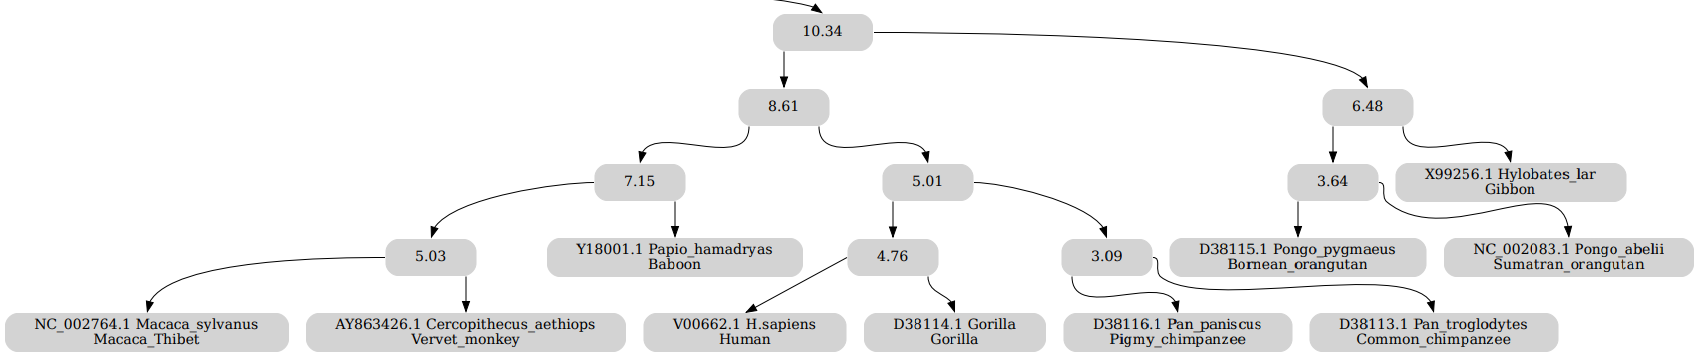
\includegraphics[width=0.8\textwidth]{images/Diferencia1.png}
  \caption{Marca la similitud entre \textit{Macaco del Tibet}, \textit{Mono Verde}, \textit{Babuino}, \textit{Humano}, \textit{Gorila}, \textit{Chimpancé Pigmeo}, \textit{Chimpancé Común}, \textit{Orangután Borneo}, \textit{Orangután de Sumatra} y el \textit{Gibón}}
\end{figure}

\begin{figure}[h!]
  \centering
  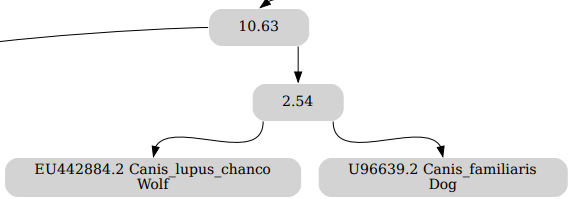
\includegraphics[width=0.5\textwidth]{images/Diferencia2.png}
  \caption{Marca la similitud entre \textit{Perros} y \textit{Lobos}}
\end{figure}

\begin{figure}[h!]
  \centering
  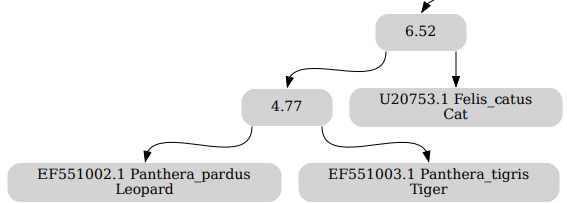
\includegraphics[width=0.6\textwidth]{images/Diferencia3.png}
  \caption{Marca la similitud entre \textit{Leopardos}, \textit{Tigres} y \textit{Gatos}}
\end{figure}

\begin{figure}[h!]
  \centering
  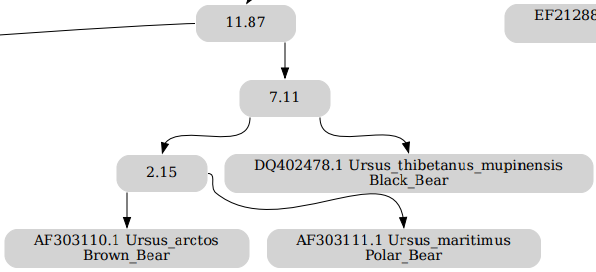
\includegraphics[width=0.6\textwidth]{images/Diferencia4.png}
  \caption{Marca la similitud entre \textit{Osos Cafés}, \textit{Osos Negros} y \textit{Osos Polares}}
\end{figure}

\newpage
Dejándonos con todas las demás especies con diferencias claras entre ellas dadas por la distancia a la que se encuentran, es decir, existen muy pocas similitudes . Por ejemplo, podemos decir que un \textit{Humano} y un \textit{Oso Polar} no son similares, pues la distancia entre ellos es más larga.
%\mbox{~}
\newpage

\subsection{Bacterias}

\begin{center}
  \href{https://gitlab.com/pppkizbroutle/proyecto-genomica/-/raw/master/src/output/bacteria.pdf?inline=false}{Resultado completo de las pruebas en bacterias}\\
  Ubicado en \texttt{src/output/bacterias.pdf} dentro del repositorio.
\end{center}

\noindent La siguiente es una tabla con cada una de las bacterias analizadas y la respectiva familia a la que pertenecen.

\begin{table}[h!]
  \centering
  \caption{Bacterias y sus respectivas familias.}
  \begin{tabular}{| c | c |}%chktex-file 44
    \hline
    Familia & Especie\\
    \hline
    \cellcolor{VioletRed}& Aeromonas hydrophila strain AHNIH1
    \\
    \cline{2-2}
    \cellcolor{VioletRed}& Aeromonas hydrophila strain GYK1\\
    \cline{2-2}
    \cellcolor{VioletRed}& Aeromonas hydrophila YL17\\
    \cline{2-2}
    \cellcolor{VioletRed}& Aeromonas veronii strain AVNIH1\\
    \cline{2-2}
    \cellcolor{VioletRed}\multirow{-5}{*}{\textit{Aeromonadaceae}}& Aeromonas veronii strain TH0426\\
    \hline
    \cellcolor{Orchid}& Bacillus anthracis str. A0248\\
    \cline{2-2}
    \cellcolor{Orchid}& Bacillus anthracis str. A16R\\
    \cline{2-2}
    \cellcolor{Orchid}& Bacillus anthracis str. Ames\\
    \cline{2-2}
    \cellcolor{Orchid}& Bacillus anthracis str. CDC 684\\
    \cline{2-2}
    \cellcolor{Orchid}& Bacillus anthracis str. H9401\\
    \cline{2-2}
    \cellcolor{Orchid}& Bacillus anthracis str. Sterne\\
    \cline{2-2}
    \cellcolor{Orchid}\multirow{-7}{*}{\textit{Bacillaceae}}& Bacillus cereus E33L\\
    \hline
    \cellcolor{Periwinkle}& Bordetella bronchialis strain AU17976\\
    \cline{2-2}
    \cellcolor{Periwinkle}& Bordetella bronchiseptica 253\\
    \cline{2-2}
    \cellcolor{Periwinkle}\multirow{-3}{*}{\textit{Alcaligenaceae}}& Bordetella flabilis strain AU10664\\
    \hline
    \cellcolor{Goldenrod}& Borrelia duttonii Ly\\
    \cline{2-2}
    \cellcolor{Goldenrod}& Borrelia hermsii DAH\\
    \cline{2-2}
    \cellcolor{Goldenrod}& Borrelia recurrentis A1\\
    \cline{2-2}
    \cellcolor{Goldenrod}\multirow{-4}{*}{\textit{Borreliaceae}}& Borrelia turicatae 91E135\\
    \hline
    \cellcolor{Aquamarine}& Phenylobacteriumzucineum HLK1\\
    \cline{2-2}
    \cellcolor{Aquamarine}& Caulobacter crescentus CB15\\
    \cline{2-2}
    \cellcolor{Aquamarine}\multirow{-3}{*}{\textit{Caulobacteraceae}}& Caulobacter crescentus NA1000\\
    \hline
    \cellcolor{Salmon}& Clostridium perfringens ATCC 13124\\
    \cline{2-2}
    \cellcolor{Salmon}& Clostridium perfringens SM101\\
    \cline{2-2}
    \cellcolor{Salmon}\multirow{-3}{*}{\textit{Clostridiaceae}}& Clostridium perfringens str. 13 DNA\\
    \hline
    \cellcolor{RedOrange}& Desulfovibrio vulgaris DP4\\
    \cline{2-2}
    \cellcolor{RedOrange}& Desulfovibrio vulgaris Hildenborough\\
    \cline{2-2}
    \cellcolor{RedOrange}\multirow{-3}{*}{\textit{Desulfovibrionaceae}}& Desulfovibrio vulgaris RCH1\\
    \hline
    \cellcolor{CadetBlue}& Erwinia pyrifoliae DSM 12163\\
    \cline{2-2}
    \cellcolor{CadetBlue}& Erwinia sp. Ejp617\\
    \cline{2-2}
    \cellcolor{CadetBlue}\multirow{-3}{*}{\textit{Erwiniaceae}}& Erwinia tasmaniensis strain ET1\--99\\
    \hline
    \cellcolor{Tan}& Lactobacillus acidophilus NCFM\\
    \cline{2-2}
    \cellcolor{Tan}& Lactobacillus helveticus DPC 4571\\
    \cline{2-2}
    \cellcolor{Tan}\multirow{-3}{*}{\textit{Lactobacillaceae}}& Lactobacillus johnsonii NCC 533\\
    \hline
    \cellcolor{Melon}& Mycoplasma agalactiae PG2\\
    \cline{2-2}
    \cellcolor{Melon}& Mycoplasma conjunctivae HRC-581T\\
    \cline{2-2}
    \cellcolor{Melon}\multirow{-3}{*}{\textit{Mycoplasmataceae}}& Mycoplasma fermentans JER\\
    \hline
    \cellcolor{Thistle}& Ralstoniaeutropha H16\\
    \cline{2-2}
    \cellcolor{Thistle}\multirow{-2}{*}{\textit{Burkholderiaceae}}& Ralstoniaeutropha JMP134\\
    \hline
    \cellcolor{OrangeRed}& Rhodobactersphaeroides 2.4.1\\
    \cline{2-2}
    \cellcolor{OrangeRed}& Rhodobactersphaeroides ATCC 17029\\
    \cline{2-2}
    \cellcolor{OrangeRed}\multirow{-3}{*}{\textit{Rhodobacteraceae}}& Rhodobactersphaeroides KD131\\
    \hline
  \end{tabular}
\end{table}

\begin{table}[h!]
  \centering
  \caption{Bacterias y sus respectivas familias (continuación)}
  \begin{tabular}{| c | c |}
    \hline
    \cellcolor{SpringGreen}& Staphylococcus carnosus subsp.\ carnosus TM300\\
    \cline{2-2}
    \cellcolor{SpringGreen}& Staphylococcus epidermidis ATCC 12228\\
    \cline{2-2}
    \cellcolor{SpringGreen}& Staphylococcus epidermidis RP62A\\
    \cline{2-2}
    \cellcolor{SpringGreen}& Staphylococcus haemolyticus JCSC1435 DNA\\
    \cline{2-2}
    \cellcolor{SpringGreen}\multirow{-5}{*}{\textit{Staphylococcaceae}}& Staphylococcus lugdunensis HKU09-01\\
    \hline
    \cellcolor{Orange}& Yersinia pestis Antiqua\\
    \cline{2-2}
    \cellcolor{Orange}& Yersinia pestis CO92\\
    \cline{2-2}
    \cellcolor{Orange}& Yersinia pestis D106004\\
    \cline{2-2}
    \cellcolor{Orange}& Yersinia pestis KIM10+\\
    \cline{2-2}
    \cellcolor{Orange}\multirow{-5}{*}{\textit{Yersiniaceae}}& Yersinia pestis Z176003\\
    \hline
    \cellcolor{Yellow}& Escherichia coli ABU 83972\\
    \cline{2-2}
    \cellcolor{Yellow}& Escherichia coli APEC O1\\
    \cline{2-2}
    \cellcolor{Yellow}& Escherichia coli ATCC 8739\\
    \cline{2-2}
    \cellcolor{Yellow}& Escherichia coli BL21\\
    \cline{2-2}
    \cellcolor{Yellow}& Shigella flexneri 2002017\\
    \cline{2-2}
    \cellcolor{Yellow}& Shigella flexneri 2a str. 301\\
    \cline{2-2}
    \cellcolor{Yellow}\multirow{-7}{*}{\textit{Enterobacteriaceae}}& Shigella sonnei Ss046\\
    \hline
  \end{tabular}
\end{table}

Y en el árbol filogenético podemos diferenciar a éstas familias, así como también ver el parecido que tienen unas con otras.

Veamos el ejemplo con las tres primeras familias en la tabla:

\begin{figure}[h!]
  \centering
  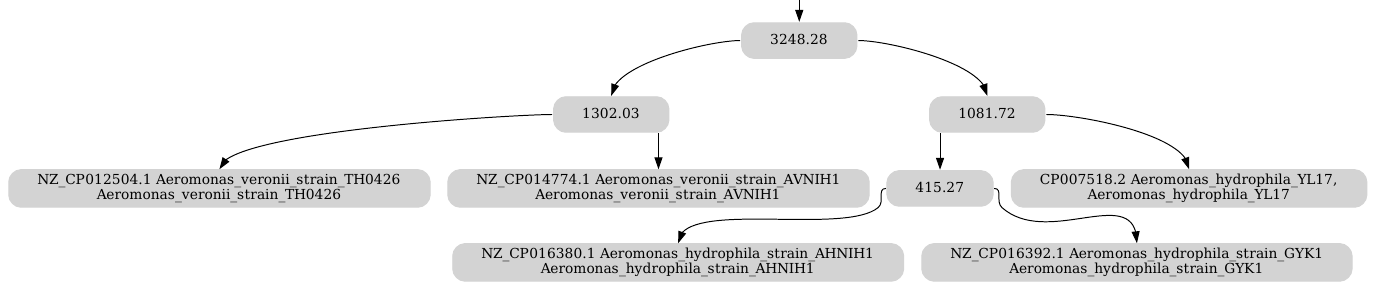
\includegraphics[width=0.8\textwidth]{Aeromonadaceae}
  \caption{Familia \textit{Aeromonadaceae} identificada en un único clúster}
\end{figure}

\begin{figure}[h!]
  \centering
  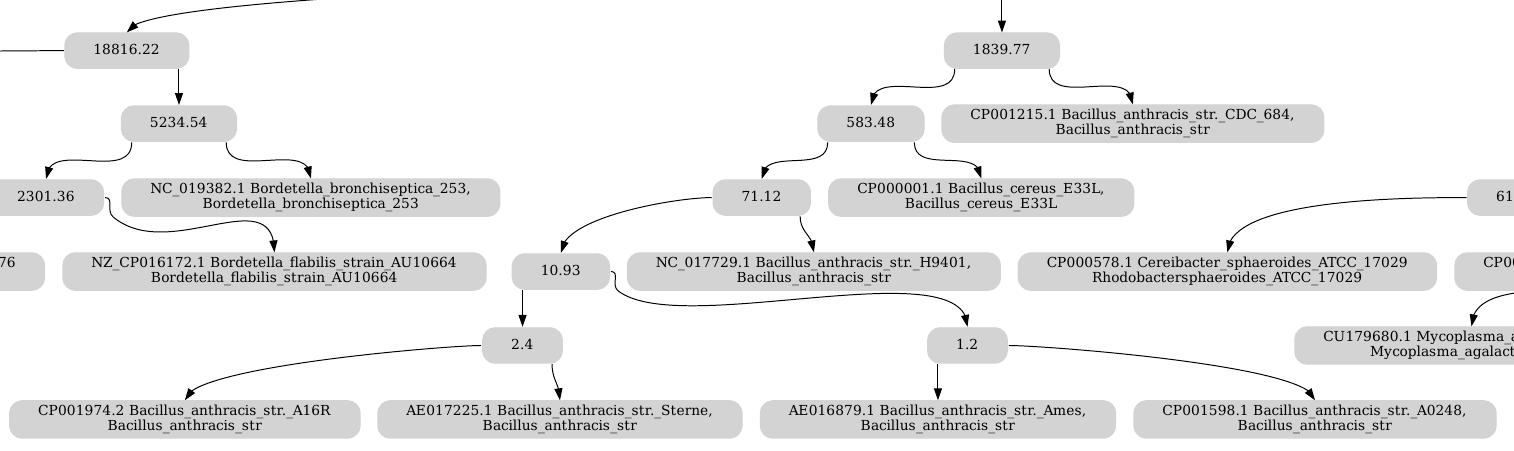
\includegraphics[width=0.8\textwidth]{Bacillaceae}
  \caption{Familia \textit{Bacillaceae} identificada en un único clúster}
\end{figure}

\begin{figure}[h!]
  \centering
  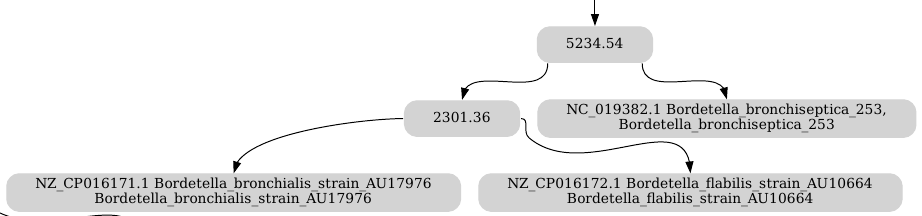
\includegraphics[width=0.8\textwidth]{Alcaligenaceae}
  \caption{Familia \textit{Alcaligenaceae} identificada en un único clúster}
\end{figure}

\newpage

\section{Conclusión}

\noindent Generar la matriz de distancias es un paso muy importante para el análisis filogenético de las especies, y los métodos que la calculan por medio de algoritmos de alineamiento pueden resultar útiles para obtener información precisa entre pocas secuencias que se requieran analizar; sin embargo, si se requiere procesar una gran cantidad de información, el uso de éste método se vuelve inviable debido principalmente a su complejidad computacional.

Por ésta razón se vuelve necesario investigar métodos que prescindan del algoritmo de alineamiento, y el acercamiento a este problema por medio de gráficas bipartitas resulta en una solución que además de mejorar el tiempo de analizar cada secuencia a lineal, también es precisa para el cálculo de distancias como vimos en los resultados. Por lo que el uso de éste método puede ser de gran utilidad para procesar una gran cantidad de datos.

\section{Datos}

La lista completa de los datos utilizados en las pruebas se encuentran en el siguiente \href{https://gitlab.com/pppkizbroutle/proyecto-genomica/-/raw/master/src/input/datos.txt}{link}.

\begin{center}
  \textit{Se encuentra en la carpeta }\texttt{src/input/datos}\textit{ del repositorio}
\end{center}

\section{Bibliografía}

\begin{enumerate}
\item Das, S., Das, A., Bhattacharya, D. \& Tibarewala, D. (2020). A new graph-theoretic approach to determine the similarity of genome sequences based on nucleotide triplets. \textit{Genomics}, 112(6), 4701\--4714.\\ \href{https://www.sciencedirect.com/science/article/pii/S088875431930638X}{https://www.sciencedirect.com/science/article/pii/S088875431930638X}
\item Das, S., Deb, T., Dey, N., Ashour, A. S., Bhattacharya, D. \& Tibarewala, D. (2018). Optimal choice of k-mer in composition vector method for genome sequence comparison. \textit{Genomics}, 110(5), 263\--273.\\ \href{https://www.sciencedirect.com/science/article/pii/S0888754317301453}{https://www.sciencedirect.com/science/article/pii/S0888754317301453}
\item Wikipedia contributors. (2022, 16 octubre). \textit{UPGMA}. Wikipedia.\\ \href{https://en.wikipedia.org/wiki/UPGMA}{https://en.wikipedia.org/wiki/UPGMA}
\end{enumerate}

\end{document}
